\chapter{Giới thiệu chung}\label{chap:intro}

\section{Bối cảnh nghiên cứu}
Việc kèm từng học sinh là một trong những can thiệp giáo dục hiệu quả nhất được biết đến: Bloom ước lượng nhóm học với gia sư vượt nhóm học theo lớp khoảng hai độ lệch chuẩn~\cite{bloom1984}, và các hệ thống gia sư thông minh hỗ trợ theo từng bước cho hiệu quả gần với gia sư người~\cite{vanlehn2011}. Lớp học đông người không cho phép giáo viên theo sát từng em. Một học sinh lớp 5 gặp khó với số thập phân hay công thức diện tích thường cần được hỏi lại, được gợi ý đúng chỗ vướng và được tự nói ra cách làm, và mỗi việc đó đòi hỏi nhiều thời gian hơn một tiết học theo lớp có thể dành cho từng em. Gia sư tự động vì vậy là công cụ bổ trợ, trong đó giáo viên vẫn giữ vai trò định hướng nội dung và theo dõi tiến bộ.

Mô hình ngôn ngữ lớn làm chi phí xây dựng một gia sư biết trò chuyện giảm mạnh~\cite{kasneci2023}, nhưng thách thức của nó mang tính sư phạm hơn là kỹ thuật. Mô hình có xu hướng đưa đáp án hoặc làm hộ bài khi học sinh yêu cầu~\cite{macina2023,tack2022}, có thể chấm sai câu trả lời, không biết học sinh đang ở đâu trong chương trình và có thể bị câu lệnh như ``bỏ qua mọi hướng dẫn trước đó'' vô hiệu hóa lời nhắc~\cite{perez2022}. Bằng chứng thực nghiệm cho thấy cách thiết kế quyết định kết quả: quyền dùng GPT-4 không ràng buộc cải thiện điểm luyện tập nhưng làm điểm kiểm tra sau đó kém đi, còn lời nhắc theo kiểu gia sư giảm phần lớn tác hại~\cite{bastani2025}; gia sư AI thiết kế theo nguyên tắc sư phạm giúp sinh viên học tốt hơn lớp học tích cực~\cite{kestin2025}. Giá trị của gia sư AI vì vậy phụ thuộc vào cách thiết kế chứ không phụ thuộc vào việc có dùng mô hình ngôn ngữ hay không.

Toán lớp 5 là lúc học sinh chuyển từ phân số sang số thập phân và làm quen công thức diện tích. Hai nội dung này có nhiều lỗi quan niệm quen thuộc, chẳng hạn trẻ coi $0{,}25$ lớn hơn $0{,}3$ vì $25$ lớn hơn $3$, hoặc nhầm đường cao với cạnh bên của hình thang; một gia sư hữu ích phải phản hồi đúng vào lỗi đó thay vì chỉ báo đúng hay sai. Tiếng Việt đặt thêm yêu cầu riêng: dấu phẩy là dấu thập phân nên $0{,}9$ và $0.9$ cùng chỉ một số nhưng chỉ cách viết thứ nhất theo chuẩn Việt Nam, và trẻ thường viết số bằng chữ (``không phẩy chín''), viết tắt không dấu hoặc thêm từ đệm. Bộ chấm theo chuẩn quốc tế dễ bác nhầm các câu đúng ở dạng này (Mục~\ref{sec:eval-grading}). Cuối cùng, đồ án do một sinh viên thực hiện cùng trợ lý lập trình AI với mục tiêu tạo sản phẩm nội bộ để kiểm thử, nên hệ thống ưu tiên dịch vụ miễn phí, mã nguồn mở và chạy cục bộ; hạn mức của dịch vụ miễn phí vì thế là một yêu cầu thiết kế (Mục~\ref{sec:nfr}).

\section{Các hướng tiếp cận hiện nay và khoảng trống}
Hệ thống gia sư thông minh truyền thống tách kiến thức chuyên môn, mô hình người học và chiến lược dạy thành các thành phần riêng. AutoTutor dẫn dắt học sinh qua hội thoại theo kịch bản soạn trước~\cite{graesser2005}, còn truy vết tri thức ước lượng xác suất học sinh đã nắm kỹ năng từ chuỗi câu trả lời~\cite{corbett1995,piech2015}. Hành vi sư phạm của dòng này kiểm soát được, nhưng chi phí soạn kịch bản cao và khó mở rộng ra câu hỏi ngoài kịch bản.

Các công trình gần đây dùng mô hình ngôn ngữ để hội thoại linh hoạt hơn. MathDial xây dựng tập hội thoại dạy Toán~\cite{macina2023}, SocraticLM tinh chỉnh mô hình để dạy theo phương pháp Socratic~\cite{liu2024socratic}, và Chowdhury cùng cộng sự kết hợp mô hình với khung hội thoại AutoTutor~\cite{chowdhury2024}. Các nhà cung cấp lớn có chế độ học riêng: study mode của ChatGPT là bộ chỉ dẫn hệ thống tùy biến~\cite{studymode}, Guided Learning của Gemini dựa trên họ LearnLM~\cite{guidedlearning,jurenka2024}, và Khanmigo gắn GPT-4 với kho bài của Khan Academy~\cite{khanmigo}.

Các cách làm này có chung đặc điểm: mô hình ngôn ngữ vẫn là nơi quyết định, còn ràng buộc sư phạm chỉ là lời khuyên trong ngữ cảnh hoặc trọng số đã tinh chỉnh. Khi lời khuyên bị bỏ qua, chẳng hạn trẻ khăng khăng một đáp án sai hoặc nhờ làm hộ, không cơ chế nào bảo đảm hành vi đúng. Từ đó có ba khoảng trống. Về kiểm soát, chưa có cơ chế tách quyết định sư phạm khỏi quá trình sinh ngôn ngữ nên khó chứng minh bất biến như không lộ đáp án. Về nền tảng nội dung, kiến thức của gia sư là kiến thức chung của mô hình, không bám tài liệu giáo viên và không biết ranh giới giữa bài đang học với bài sắp học. Về đánh giá, mức hiểu bài thường suy ra từ phản hồi do mô hình tạo nên khó tái lập và khó kiểm toán.

\section{Vấn đề nghiên cứu, mục tiêu và phạm vi}
Vấn đề nghiên cứu là làm thế nào xây dựng một gia sư Toán tiếng Việt dùng mô hình ngôn ngữ lớn nhưng vẫn bảo đảm các hành vi sư phạm bất biến: không lộ đáp án khi đang kiểm tra, chấm đúng theo chuẩn viết số Việt Nam, không dạy trước nội dung bài sau và ghi mức hiểu bài theo cách tái lập được, trong giới hạn dịch vụ miễn phí và dạy từ tài liệu của chính giáo viên. Mục tiêu của đồ án là thiết kế, hiện thực và đánh giá một kiến trúc dựng hệ thống học tập trước và giao cho mô hình ngôn ngữ một vai trò hẹp bên trong, cụ thể hóa thành năm quyết định. Một chính sách tất định (cùng đầu vào luôn cho cùng kết quả, không có yếu tố ngẫu nhiên) và có phiên bản chọn từng nước đi sư phạm; mô hình chỉ chuyển nước đi thành lời và lời đó phải qua bộ kiểm chứng. Một bộ chấm tất định quyết định đúng sai, và đáp án câu kiểm tra không nằm trong ngữ cảnh gửi cho mô hình. Mức hiểu bài là kết quả của một phép tính tất định (gọi là phép chiếu) trên sổ sự kiện, tức nhật ký chỉ được ghi thêm, không bị sửa, nên có thể tính lại bất cứ lúc nào. Kiến thức của gia sư là tài liệu của giáo viên, được đọc, kiểm đáp án và dựng thành đồ thị tri thức để truy xuất có ràng buộc. Một bộ chọn contextual bandit chọn nước đi trong tập nước đi mà chính sách cho phép mà không đổi các bất biến trên. Hình~\ref{fig:two-designs} đối chiếu cách này với cách để mô hình tự quyết định mọi việc.

\begin{figure}[H]
\centering
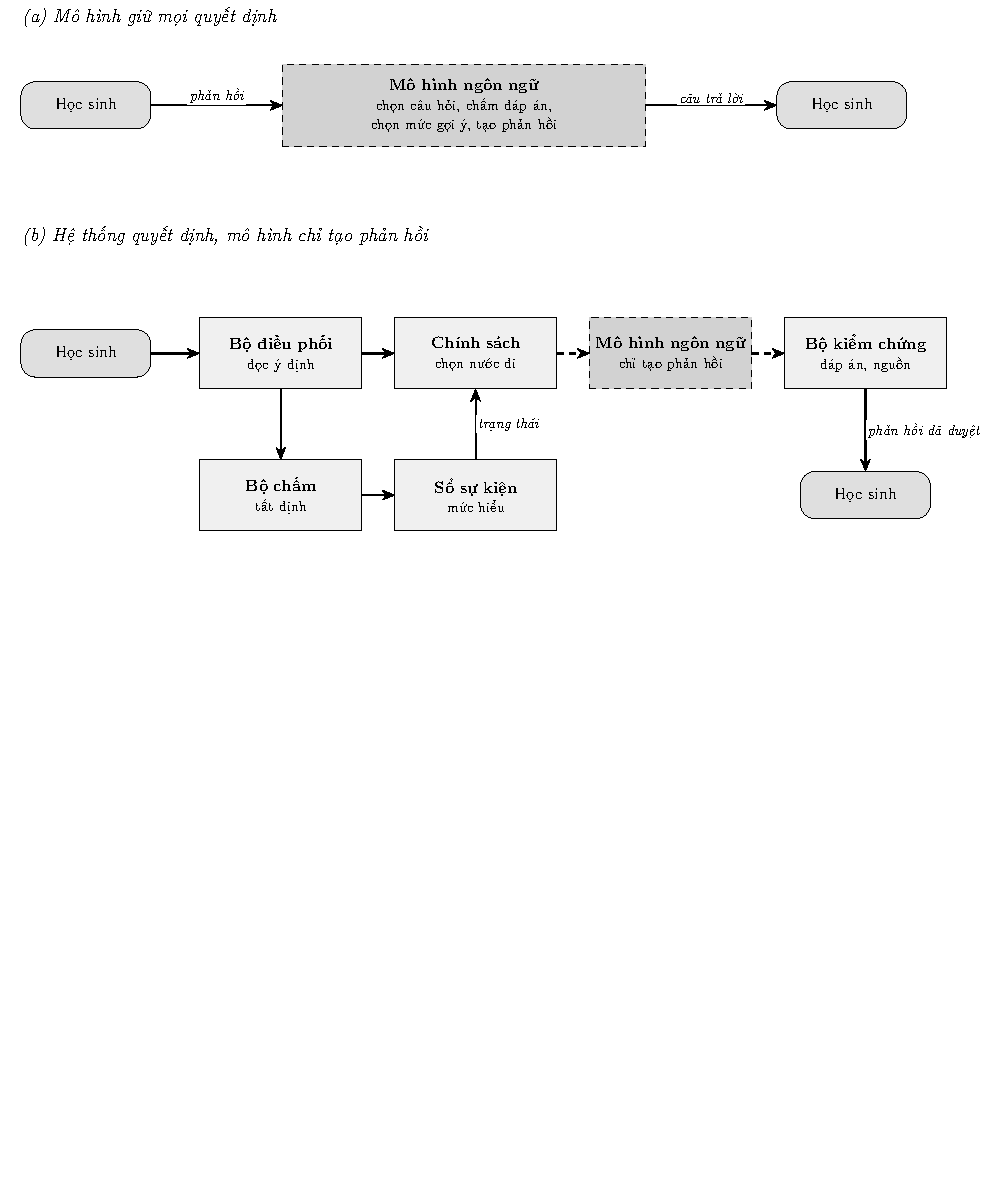
\includegraphics[width=\linewidth]{figures/pdf/fig-two-designs.pdf}
\caption{Hai cách đặt mô hình ngôn ngữ trong một gia sư. Đồ án theo cách (b). Hình bầu dục: học sinh; hình chữ nhật: thành phần xử lý; nét đứt: phần do mô hình ngôn ngữ thực hiện.}
\label{fig:two-designs}
\end{figure}

Đối tượng chính là học sinh lớp 5; giáo viên duyệt nội dung và xem bằng chứng học tập, phụ huynh xem tiến bộ của con. Nội dung khóa ở hai chương Toán lớp 5, ``Số thập phân'' và ``Diện tích hình tam giác, hình thang'', với 19 tiết dựng từ 18 tệp tài liệu giáo viên (77 trang). Học sinh nhập văn bản hoặc nói với gia sư; nhận dạng tiếng nói dùng Whisper trên Groq và giọng gia sư dùng VieNeu-TTS chạy cục bộ. Hệ thống chỉ gọi mô hình ngôn ngữ qua một cổng AI và không dùng khung RAG hay tác tử có sẵn: truy xuất, đồ thị tri thức, chấm điểm và chính sách dạy đều tự xây dựng. Đồ án không nghiên cứu hiệu quả học tập dài hạn trên học sinh thật và không xét vấn đề pháp lý về dữ liệu trẻ em.

\section{Câu hỏi nghiên cứu và phương pháp}
Đồ án đặt năm câu hỏi nghiên cứu, nêu ở Bảng~\ref{tab:rq} cùng chỉ số chính và nơi trả lời. Phương pháp theo hướng nghiên cứu thiết kế: đề xuất kiến trúc, hiện thực thành hệ thống chạy được rồi đánh giá bằng thực nghiệm. Chỉ số nào đo được bằng luật thì đo bằng luật, còn mô hình chỉ làm giám khảo cho chất lượng ngôn ngữ và khác họ với mô hình gia sư. Mỗi bộ câu dùng để chỉnh tham số có bộ giữ riêng viết sau, và các tập đánh giá được đóng băng bằng thẻ git trước khi sửa mã mà chúng đo. Ngưỡng hay công thức không có trong khung đánh giá gốc được đánh dấu là diễn giải khai báo (DI) và chờ giáo viên duyệt. Hệ thống được đánh giá chủ yếu bằng học sinh mô phỏng, các vai khó dựng sẵn, bộ câu hỏi do người phát triển soạn và các buổi thử nghiệm bằng tài khoản Vuong, vì mục tiêu của giai đoạn này là kiểm chứng kiến trúc chứ chưa đo kết quả học tập của trẻ.

\begin{table}[H]
\centering
\caption{Các câu hỏi nghiên cứu, chỉ số chính và nơi trả lời.}
\label{tab:rq}
\small
\begin{tabularx}{\linewidth}{@{}p{1.1cm}>{\raggedright\arraybackslash}p{5.3cm}XX@{}}
\toprule
Mã & Câu hỏi & Chỉ số chính & Nơi trả lời \\
\midrule
RQ1 & Đánh giá một hệ thống như vậy bằng phương pháp và theo chiều nào? & Bộ đo tất định; giám khảo khác họ mô hình; bộ giữ riêng đóng băng & Mục~\ref{sec:eval-method} \\
RQ2 & Truy xuất có ràng buộc theo đồ thị đạt mức nào so với truy xuất phẳng? & Hit@3, MRR, số đoạn bài sau lọt vào kết quả đầu & Mục~\ref{sec:eval-rag} \\
RQ3 & Gia sư hỗ trợ học sinh hơn chatbot thông thường ở điểm nào? & Số lượt lộ đáp án, câu hỏi mỗi lượt, độ dài; độ đúng của bộ chấm & Mục~\ref{sec:eval-socratic}, \ref{sec:eval-grading} \\
RQ4 & Cách ước lượng mức hiểu sát khung đánh giá đến đâu? & Số mục khung đã hiện thực; độ lệch công thức; độ nhạy & Mục~\ref{sec:eval-learner} \\
RQ5 & Bộ chọn nước đi học được nhanh đến đâu và nhật ký có đủ để đánh giá chính sách khác không? & Hối tiếc tích lũy; sai lệch ước lượng IPS & Mục~\ref{sec:eval-bandit} \\
\bottomrule
\end{tabularx}
\end{table}

\section{Đóng góp và bố cục}
Đồ án có năm đóng góp. Thứ nhất, kiến trúc tách quyết định sư phạm khỏi mô hình ngôn ngữ với sáu bất biến thiết kế, mỗi bất biến gắn với thành phần bảo đảm và phép kiểm chứng riêng (Bảng~\ref{tab:invariants}). Thứ hai, phương pháp truy xuất lai có ràng buộc theo đồ thị tri thức, giữ độ chính xác ngang truy xuất phẳng và loại kiến thức bài sau khỏi kết quả đầu. Thứ ba, mô hình người học tất định, có phiên bản, phát lại được từ sổ sự kiện, cùng bộ chấm theo chuẩn viết số Việt Nam. Thứ tư, quy trình đưa tài liệu giáo viên thành phương án dạy: đọc từng trang, kiểm đáp án, dựng đồ thị tri thức, soạn phần còn thiếu và chỉ dạy bản đã được giáo viên duyệt. Thứ năm, bộ chọn nước đi bằng LinUCB trên tập nước đi do chính sách cho phép, có trạng thái tính lại được và ghi xác suất từng lượt chọn để đánh giá ngoài chính sách. Đồ án để lại một hệ thống chạy được dưới tên Monkey Edu với giao diện cho học sinh, phụ huynh và giáo viên, tương tác bằng giọng nói và gói triển khai Docker.

Đồ án gồm bốn chương và một mục Kết luận. Chương~\ref{chap:theory} trình bày cơ sở lý thuyết. Chương~\ref{chap:design} phân tích yêu cầu, nêu các bất biến và mô tả kiến trúc cùng thiết kế từng thành phần. Chương~\ref{chap:eval} trình bày phương pháp đánh giá và kết quả trên dữ liệu thử nghiệm thực tế và các bộ câu hỏi đã đóng băng. Mục Kết luận tổng kết kết quả, hạn chế và hướng phát triển.
